\documentclass[10pt,twocolumn,letterpaper]{article}

\usepackage{iccv}
\makeatletter
\@namedef{ver@everyshi.sty}{}
\makeatother
\usepackage{tikz}
\usepackage{listings}
\usepackage{times}
\usepackage{epsfig}
\usepackage{graphicx}
\usepackage{calc}
\usepackage{amsmath}
\usepackage{amssymb}
\usepackage{tabu}
\usepackage{adjustbox}
\usepackage[percent]{overpic}
\usepackage[utf8]{inputenc}
\usepackage{pgfplots}
\DeclareUnicodeCharacter{2212}{−}
\usepgfplotslibrary{groupplots,dateplot}
\usetikzlibrary{patterns,shapes.arrows}
\pgfplotsset{compat=newest}

\definecolor{codegreen}{rgb}{0,0.6,0}
\definecolor{codegray}{rgb}{0.5,0.5,0.5}
\definecolor{codepurple}{rgb}{0.58,0,0.82}
\definecolor{backcolour}{rgb}{0.95,0.95,0.92}

\lstdefinestyle{mystyle}{
  backgroundcolor=\color{backcolour},
  commentstyle=\color{codegreen},
  keywordstyle=\color{magenta},
  numberstyle=\tiny\color{codegray},
  stringstyle=\color{codepurple},
  basicstyle=\ttfamily\footnotesize,
  breakatwhitespace=false,         
  breaklines=true,                 
  captionpos=b,                    
  keepspaces=true,                 
  numbers=left,                    
  numbersep=5pt,                  
  showspaces=false,                
  showstringspaces=false,
  showtabs=false,                  
  tabsize=2
}

\lstset{style=mystyle}

\usetikzlibrary{decorations.pathreplacing,calc,automata, shapes.geometric,shapes.arrows,decorations.pathmorphing,matrix,chains,scopes,positioning,arrows,fit}

\newcommand{\tikzmark}[2][-3pt]{\tikz[remember picture, overlay, baseline=-0.5ex]\node[#1](#2){};}


\usepackage[pagebackref=true,breaklinks=true,letterpaper=true,colorlinks,bookmarks=false]{hyperref}

\iccvfinalcopy %

\def\iccvPaperID{xxxx} %
\def\httilde{\mbox{\tt\raisebox{-.5ex}{\symbol{126}}}}


\definecolor{purple}{rgb}{1, 0, 1}

\newcommand{\ie}{\emph{i.e.,}\xspace}
\newcommand{\eg}{\emph{e.g.,}\xspace}
\newcommand{\abr}{\emph{abbr.}\xspace}
\newcommand{\ea}{\emph{et al.}\xspace}
\newcommand{\gensync}{\emph{GenSync}\xspace}
\newcommand{\colosseum}{\emph{Colosseum}\xspace}
\newcommand{\srep}{\emph{SREP}\xspace} % Set Reconciliation Enhances
\newcommand{\srepsim}{\emph{SREPSim}\xspace}
% Propagation
\newcommand{\esrep}{\emph{E-SREP}\xspace}
\newcommand{\epsrep}{\emph{EP-SREP}\xspace}
\newcommand{\mesrep}{\emph{ME-SREP}\xspace}
\newcommand{\mempoolsync}{\emph{MempoolSync}}

\newcommand{\fref}[1]{Fig.~\ref{#1}}
\newcommand{\tref}[1]{Table~\ref{#1}}
\newcommand{\aref}[1]{Algorithm~\ref{#1}}
\newcommand{\procref}[1]{Procedure~\ref{#1}}
\newcommand{\sref}[1]{Section~\ref{#1}}
\newcommand{\lineref}[1]{line~\ref{#1}}
\newcommand{\appref}[1]{Appendix~\ref{#1}}

% Change \eqref
\LetLtxMacro{\originaleqref}{\eqref}
\renewcommand{\eqref}{Eq.~\originaleqref}

% Theorems and corollaries
\newcounter{theoremcount}
\setcounter{theoremcount}{0}
\DeclareRobustCommand{\theorem}[1]{%
  \refstepcounter{theoremcount}%
  \noindent\textit{\textbf{Theorem \thetheoremcount\label{theorem:#1}: }}%
}
\DeclareRobustCommand{\theoremref}[1]{Theorem~\ref{theorem:#1}}

\DeclareRobustCommand{\proof}{\emph{Proof:}\xspace}
\DeclareRobustCommand{\qqed}{\hfill$\blacksquare$}

\newcounter{corollcount}
\setcounter{corollcount}{0}
\DeclareRobustCommand{\coroll}[1]{%
  \refstepcounter{corollcount}%
  \noindent\textit{\textbf{Corollary \thecorollcount\label{coroll:#1}: }}%
}
\DeclareRobustCommand{\corollref}[1]{Corollary~\ref{coroll:#1}}

\newcounter{lemmacount}
\setcounter{lemmacount}{0}
\DeclareRobustCommand{\lemma}[1]{%
  \refstepcounter{lemmacount}%
  \noindent\textit{\textbf{Lemma \thelemmacount\label{lemma:#1}: }}%
}
\DeclareRobustCommand{\lemmaref}[1]{Lemma~\ref{lemma:#1}}

\newcounter{definitioncount}
\setcounter{definitioncount}{0}
\DeclareRobustCommand{\definition}[1]{%
  \refstepcounter{definitioncount}%
  \noindent\textit{\textbf{Definition \thedefinitioncount\label{definition:#1}: }}%
}
\DeclareRobustCommand{\defref}[1]{Definition~\ref{definition:#1}}

%notes of different authors
\newif\ifnotes
\notestrue
\notesfalse

\newif\ifdiff
\difftrue
\difffalse

\newcommand{\anote}[1]{\ifnotes $\ll$\textsf{\textcolor{purple}{Ari: {#1}}}$\gg$ \fi}
\newcommand{\nnote}[1]{\ifnotes $\ll$\textsf{\textcolor{orange}{Novak: {#1}}}$\gg$ \fi}
\newcommand{\diff}[1]{\ifdiff\textcolor{orange}{#1}\else#1\fi}

%%% Local Variables:
%%% mode: latex
%%% TeX-master: "main"
%%% End:


\begin{document}

\title{Point2Vec for Self-Supervised Representation Learning on Point Clouds\vspace{-15pt}}

\newcommand{\footremember}[2]{%
   \thanks{#2}
    \newcounter{#1}
    \setcounter{#1}{\value{footnote}}%
}
\newcommand{\footrecall}[1]{%
    \footnotemark[\value{#1}]%
} 


\author{Karim Abou Zeid\footremember{cont}{Equal contribution.}, \ \ Jonas Schult\footrecall{cont}~, \ \ Alexander Hermans, \ \ Bastian Leibe
\vspace{1px}\\
Computer Vision Group, Visual Computing Institute\\
RWTH Aachen University
\vspace{1px}\\
{\tt \small karim.abou.zeid@rwth-aachen.de \quad \{schult,hermans,leibe\}@vision.rwth-aachen.de}\\
{\tt \href{https://www.vision.rwth-aachen.de/point2vec}{vision.rwth-aachen.de/point2vec}}
}

\ificcvfinal\thispagestyle{empty}\fi
\maketitle


\begin{abstract}
% \vspace{-1em}
The diffusion-based generative models have achieved remarkable success in text-based image generation. However, since it contains enormous randomness in generation progress, it is still challenging to apply such models for real-world visual content editing, especially in videos. 
In this paper, we propose \texttt{FateZero}, a zero-shot text-based editing method on real-world videos without per-prompt training or use-specific mask. 
\RM{Specifically, different from a pipeline of two independent inversion and then generation stages, we find the intermediate attention maps during inversions store better structure and motion information. We thus reform them to temporally casual attention and replace them in the generation progress. To further reduce the unnecessary semantic leakage of source video and enhance the editing quality, we then remix the temporally casual attentions via the cross-attention features of the source prompt as the mask.}
To edit videos consistently, we propose several techniques based on the pre-trained models. Firstly, in contrast to the straightforward DDIM inversion technique, our approach captures intermediate attention maps during inversion, which effectively retain both structural and motion information. These maps are directly fused in the editing process rather than generated during denoising. To further minimize semantic leakage of the source video, we then fuse self-attentions with a blending mask obtained by cross-attention features from the source prompt. Furthermore, we have implemented a reform of the self-attention mechanism in denoising UNet by introducing spatial-temporal attention to ensure frame consistency.
Yet succinct, our method is the first one to show the ability of zero-shot text-driven video style and local attribute editing from the trained text-to-image model. We also have a better zero-shot shape-aware editing ability based on the text-to-video model~\cite{tuneavideo}. \RM{Besides video, our unified method also achieves state-of-the-art performance in zero-shot image editing.\chenyang{Need exp or remove the zero-shot image}} Extensive experiments demonstrate our superior temporal consistency and editing capability than previous works.
% The code will be released.
% \chenyang{emphasize: our observation at inversion time} \xiaodong{replacing the bold part to the actual pipeline: \textbf{Specifically, we work on replacing and mixing the attention maps between the inversion and generation since the self-attention map keeps the structure of the original natural image and the cross-attention is semantic-related, after remixing, we replace them in the corresponding generation steps for denoising.}}
% \footnote{Since there is no general video diffusion model is publicly available, we use one-shot video generation method~(Tune-A-Video~\cite{tuneavideo}) as the pretrained video diffusion model for zero-shot video editing\xiaodong{can be removed if we actually zero-shot on video}.}.
\end{abstract}
\section{Introduction}

The ability to reason about plans is critical for performing long-horizon tasks \citep{erol1996hierarchical, sohn2018hierarchical, sharma-etal-2022-skill}, compositional generalization \citep{corona-etal-2021-modular} and generalization to unseen tasks and environments \citep{shridhar2020alfred}.
Consider a simple long-horizon planning scenario where a robot is tasked with preparing a meal and serving it on the table. 
This presents a non-trivial planning problem since the agent needs to understand the sequence of operations required to perform the task and search for the relevant objects in the unfamiliar environment by interacting with various objects. %



Large language models have been recently shown to possess commonsense knowledge about the world such as object affordances and physical dynamics \citep{ouyang2022training,chowdhery2022palm}.
Early approaches considered text based environments and fine-tuned PLMs to predict actions given the history of past observations and actions \citep{jansen-2020-visually,micheli-fleuret-2021-language,yao-etal-2020-keep}.
Recent work has used this ability to reason about plans from text instructions in simulated household environments with simplifying assumptions such as text-only environment observations or feedback \citep{huang2022language,ahn2022can,li2022pre,logeswaran-etal-2022-shot}.


We focus on \emph{visually grounded planning} with PLMs --- the ability to adapt plans based on interaction and visual feedback from the environment.
While PLMs have strong planning commonsense priors, predictions from a PLM may not be directly realizable in the environment since the observation and action spaces are unknown.
This requires \emph{grounding} the PLM in the environment and adapting it to observe visual feedback, which is highly non-trivial.
Some prior works assume the availability of a pre-trained affordance function \citep{ahn2022can} or a success detector \citep{mirchandani2021ella}.
Notably, SayCan \citep{ahn2022can} completely decouples the PLM from observation information by selecting actions that have both high affordability (through a pre-trained affordance model) and high PLM likelihood.
Although this partially addresses the grounding problem, the use of visual feedback for action affordance alone is limited.
Often an agent must choose one of many affordable actions using information from observations.
For example, a driving agent should re-navigate and possibly turn around when encountering a ``road closed'' sign, but both turning around and driving forward are indistinguishable to SayCan because they are both affordable and the PLM is blind to observations.

Another workaround explored in prior work is translating the information in the visual observations to text using a pre-trained captioning system \citep{shridhar2021alfworld,huang2022language}.
However, it can be difficult to faithfully describe an image in words and information is lost in this inherently noisy process, which limits the information available to the planner.



Recent work shows that PLMs can be adapted for various natural language tasks by inserting tunable embeddings or soft prompts at the input of the PLM (also called prompt tuning or prefix tuning)~\citep{li-liang-2021-prefix,lester-etal-2021-power}.
This approach also extends to multi-modal understanding tasks such as image captioning \citep{mokady2021clipcap} and VQA \citep{tsimpoukelli2021multimodal} where images are encoded as soft prompts and finetuned for the target task.
Transformer based architectures have also been successfully applied to offline Reinforcement Learning in recent work \citep{chen2021decision,janner2021offline,li2022pre,reid2022can}.

Taking inspiration from these works, we propose the simple approach of embedding visual observations (`visual prompts') and \textit{directly inserting them as PLM input embeddings}.
The visual encoder and PLM are jointly trained for the target task, an approach we call \textbf{\oursfull}~(\ours).
By teaching the PLM to use observations for planning in an end to end manner, we remove the dependency on external data such as captions and affordability information that was used in prior work.
We show that this simple approach performs better than prior PLM-based planning approaches on two embodied planning benchmarks based on ALFWorld~\citep{shridhar2021alfworld} and Virtualhome~\cite{puig2018virtualhome}.



\section{Related Work}

\subsection{Pattern discovery on systematic AI errors}

Systematic errors, sometimes coined as blind spots or unknown-unknowns \cite{BeatMachineChallengingHumans}, refer to model's failure over a group of instances that share similar semantics. There are various approaches for discovering such patterns, including algorithmic, human, or hybrid techniques.

A number of studies have shown that fully algorithmic techniques can help automatically discover unknown-unknowns \cite{lakkaraju2017identifying, coveragebasedutility}. Recently, several studies have also been proposed to advance the methods towards discovering automatic slices or subclasses that are semantically coherent \cite{DominoDiscoveringSystematicErrorsCrossModal, SpotlightGeneralMethodDiscoveringSystematic}, or to propose a framework for evaluating blindspot discovery methods in a unified manner \cite{EvaluatingSystemicErrorDetectionMethods}.

On the other hand, researchers have also explored how human intelligence can identify blind spots where automatic techniques alone do not work. Several studies \cite{BeatMachineChallengingHumans, ContradictMachineHybridApproach, HybridHumanAIWorkflowsUnknown, InvestigatingHumanMachineComplementarity} demonstrated that a well-designed crowdsourcing study can detect problematic instances. Hybrid workflows to leverage the abilities of both humans and machines \cite{HybridHumanAIWorkflowsUnknown, lakkaraju2017identifying, han2021iterative, chung2018unknownexamples} have also been explored throughout several studies in proposing collaborative human-AI workflow \cite{HybridHumanAIWorkflowsUnknown} or generating text descriptions \cite{han2021iterative} about spurious patterns.

While these studies demonstrate how human intelligence plays a significant role, tool support is still lacking to guide practitioners to inspect, identify, and mitigate systematic errors. In our study, we provide a workflow and systematic support for inspecting which systematic errors are attributed to interpretable concepts.

\subsection{Visual analytics for ML diagnostics}
Visual analytics tools in recent years have evolved to offer interactive ways for inspecting the machine learning process. In general, these tools aim to better visualize the predictive results in a model-agnostic manner or present the structure of the model in a model-specific way. Model-agnostic approaches propose to better visualize machine learning results regardless of model types. Many visualizations among them are largely designed on the grounds of confusion matrix as tree or flow diagram \cite{shen2020designing, VisualizingSurrogateDecisionTrees}, comparative visual design \cite{ManifoldModelAgnosticFrameworkInterpretation, ExplainExploreVisualExplorationMachine, olson2021contrastive, kaul2021improvingcounterfactuals, krause2017workflow}, radial \cite{VisualMethodsAnalyzingProbabilistic} or multi-axes based layout \cite{SquaresSupportingInteractivePerformance}. On the other hand, model-specific inspections also gained attention to support the inspection of a deep neural network inside its layers, neurons, or activations \cite{liu2017analyzingtraining, ShapeShopUnderstandingDeepLearning, TopoActVisuallyExploringShape, DeepVIDDeepVisualInterpretation}.

Visual analytic tools can also help inspect and explain the potential cause of systematic failures such as a shifted or skewed distribution of the training examples termed as out-of-distribution \cite{OoDAnalyzerInteractiveAnalysisOutofDistribution}, covariate or concept shift \cite{DiagnosingConceptDriftVisual} or machine biases \cite{FairVisVisualAnalyticsDiscovering, FairSightVisualAnalyticsFairness, WhatIfToolInteractiveProbing}. The OoD analyzer \cite{OoDAnalyzerInteractiveAnalysisOutofDistribution} presented a grid-based layout to visualize the distributional differences in training and test sets. The problem of concept drift was tackled and presented as visualizations in a 2D heatmap visualization \cite{DiagnosingConceptDriftVisual} or distribution-based scatterplot \cite{ConceptExplorerVisualAnalysisConcept}. Other interactive tools such as Deblinder \cite{DiscoveringValidatingAIErrorsCrowdsourced}, SEAL \cite{SEALInteractiveToolSystematicError}, or Error Analysis \cite{erroranalysis} have recently been proposed to mitigate systematic errors with subclass labeling or user-generated report. Compared to previous work, our study aims to promote a human-in-the-loop workflow consisting of tasks to identify biased patterns and their association/attribution aspects with the perspective of spurious associations.

% Recent visualization studies also proposed how to better explain them with counterfactuals [BF-1], or to present them in a form of report [BF-3]. 


\subsection{Understanding model with concept interpretability}

The XAI methods to explain the behavior of black box models \cite{InterpretabilityFeatureAttributionQuantitative, AutomaticConceptbasedExplanations, BayesianCaseModelGenerative, ConceptWhiteningInterpretable2020} have been recently expanded to a concept-level sensitivity. The method called TCAV (Testing Concept Activation Vector) \cite{InterpretabilityFeatureAttributionQuantitative} provides a post-hoc method to explain the global influence of a concept in a pre-trained model. ACE (Automatic Concept Extraction) \cite{AutomaticConceptbasedExplanations} was proposed to identify and filter interpretable concepts from the meaningful clusters of segments on the basis of TCAV. In \cite{ConceptWhiteningInterpretable2020}, Concept Whitening (CW) purposefully alters batch normalization layers to a concept whitening layer to learn an interpretable latent space. Especially, the whitening step in this method points out that the concept space needs to be preprocessed to better align concept vectors.

These concept-level interpretability methods, however, require the human ability to observe and extract semantically meaningful concepts \cite{AutomaticConceptbasedExplanations}. There are various ways to identify and extract concepts in collaboration with humans and systems \cite{AutomaticConceptbasedExplanations, NeuroCartographyScalableAutomaticVisualSummarization, zhao2021humanintheloopextraction, DASHVisualAnalyticsDebiasingImage,  ConceptExplorerVisualAnalysisConcept, ProtoSteerSteeringDeepSequence, AnchorVizFacilitatingSemanticData, ConceptVectorTextVisualAnalytics, VisualConceptProgrammingVisualAnalytics}. ConceptExtract \cite{zhao2021humanintheloopextraction} aimed to support concept extraction and classification in a human-in-the-loop workflow and visual tools. In DASH \cite{kwon2022dash}, problematic biases from irrelevant concepts can be identified through observations from users, which were proposed to be mitigated through random image generation using GAN techniques. ConceptExplainer \cite{ConceptExplorerVisualAnalysisConcept} was designed to explore the concept associations focusing on validating conceptual overlapping between classes, especially serving as a concept exploration tool for non-expert users. In \cite{VisualConceptProgrammingVisualAnalytics}, a self-supervised technique was proposed to automatically extract visual vocabulary to allow experts to refine the labeled data and understand the concepts.

Unlike existing work, our study proposes an interactive workflow of exploring concepts for the purpose of inspecting systematic errors and spurious concept associations behind them. Similar to \cite{WhatDidMyAILearn}, our human-in-the-loop workflow aims to promote the sensemaking of practitioners specifically in the problem of systematic errors where they can iteratively work on subsetting, contrasting patterns in instances, and hypothesizing spurious associations.


% All these methods including.. share the idea of defining a concept vector with a group of semantically coherent segments. While we take the approach of pre-processing steps on concept space in [] and sensitivity, we expand the utility of concept exploration towards inspecting model's false behaviors. In our study, we demonstrate that using concept interpretability can help not only interpreting the concept association towards misclassificaitons, and tracing back ... then removing the biases to further improve the quality of classification.






\begin{figure*}[t!]
\includegraphics[width=1.0\linewidth, trim={0 0.3cm 0 0.1cm}, clip]{figures/architecture/architecture.pdf}
\vspace{-15pt}
\caption{
\textbf{Point2Vec pre-training.}
Our model divides the input point cloud into %
point patches using farthest point sampling (FPS) and $k$-NN aggregation.
We obtain patch embeddings by applying a mini-PointNet\,\colorsquare{m_pointnet} to each point patch (\emph{right}).
The teacher Transformer encoder\,\colorsquare{m_green} infers a contextualized %
representation for all patch embeddings which, after normalization and averaging over the last $K$ Transformer layers, serve as training targets.
The student's input is a masked view on the input data, \ie we randomly mask out a ratio of patch embeddings and only pass the remaining embeddings into the student Transformer encoder\,\colorsquare{m_blue}.
After applying a shallow decoder\,\colorsquare{m_red} on the outputs of the student, padded with learned mask embeddings\,\protect\maskembedding{}, we train the student and decoder to predict the latent teacher representation of the patch embeddings.
\vspace{-10pt}
}
\label{fig:model}
\end{figure*}
\section{Method}

The aim of this work is to unlock the full potential of data2vec-like\,\cite{baevski2022data2vec} pre-training on point clouds by addressing point cloud specific challenges.
To achieve this, we first summarize the technical concepts of data2vec (\refsec{method_d2v}) and show how to learn rich representations on point clouds using data2vec pre-training (\refsec{method_d2v_pcl}).
Finally, we propose \name{}, which accounts for the point cloud specific limitations of data2vec (\refsec{method_p2v}).

\subsection{Data2vec}\label{sec:method_d2v}
Data2vec\,\cite{baevski2022data2vec} is designed to pre-train Transformer-based models, which involve a feature encoder that maps the input data to a sequence of embeddings.
These embeddings are subsequently passed to a standard Transformer encoder to generate the final latent representations.
During pre-training, two versions of the Transformer encoder are kept: a \emph{student} and a \emph{teacher}.
The teacher is a momentum encoder, \ie its parameters $\Delta$ track the student's parameters $\theta$ by being updated after each training step according to an exponential moving average (EMA) rule\,\cite{caron2021dino, baevski2022data2vec, grill2020BYOL, he2020moco}: $\Delta \leftarrow \tau \Delta + (1-\tau)\theta$,
where $\tau \in [0,1]$ is the EMA decay rate.
The teacher provides the training targets, which the student predicts given a corrupted version of the same input.

In a first step, the teacher encodes the uncorrupted input sequence.
The training targets are then constructed by averaging the outputs of the last $K$ blocks of the teacher, which are normalized beforehand to prevent a single block from dominating the sum.
Due to the self-attention layers, these targets are \emph{contextualized}, \ie they incorporate global information from the whole input sequence.
This is an important difference to other masked-prediction methods such as BERT\,\cite{devlin2018bert} and MAE\,\cite{he2022mae}, where the targets only comprise local information, \eg a word or an image patch. %

The student is given a masked version of the same input, where some of the embeddings in the input sequence are substituted by a special learned \emph{mask embedding}. %
The student's task is to predict the targets corresponding to the masked parts of the input.
The model is trained by optimizing a Smooth L1 loss on the regressed targets. %







\subsection{Data2vec for Point Clouds}\label{sec:method_d2v_pcl}

To apply data2vec to point clouds, we utilize the same underlying model as Point-BERT\,\cite{yu2021pointbert} and Point-MAE\,\cite{pang2022pointmae}.
This model is well suited for data2vec pre-training: it extracts a sequence of patch embeddings from the input point cloud and feeds it to a standard Transformer encoder.
For downstream tasks, we append a task-specific head to the Transformer encoder (\refsec{experiments}).
Next, we describe the point cloud embedding and the Transformer in detail and conclude with a summary of data2vec for point clouds.


\parag{Point Cloud Embedding.}
First, we sample $n$ center points from the input point cloud using farthest point sampling (FPS)\,\cite{qi2017pointnetplusplus}.
Grouping the center points' $k$-nearest neighbors ($k$-NN) in the point cloud yields $n$ contiguous \emph{point patches}, \ie sub-clouds of $k$ elements.
Next, we normalize the point patches by subtracting the corresponding center point from the patch's points.
This untangles the positional and the structural information.
To account for the permutation-invariant property of point clouds, we employ a mini-PointNet\,\cite{qi2016pointnet} (\reffig{model}, \emph{right}) that maps each normalized point patch to a \emph{patch embedding}.

The mini-PointNet involves the following steps:
First, we map each point of a patch to a feature vector using a shared MLP.
Then, we concatenate max-pooled features to each feature vector.
The resulting feature vectors are then passed through a second shared MLP and a final max-pooling layer to obtain the patch embedding.

\paragraph{Transformer Encoder.}
The central component of the model is a standard Transformer encoder.
The patch embeddings form the input sequence to the Transformer encoder.
Since the point patches are normalized, the patch embeddings carry no positional information;
therefore, a two-layer MLP maps each center point to a position embedding, which is then added to the corresponding patch embedding.
Due to the special importance of positional information in point clouds, the position embeddings are added again before each subsequent Transformer block to ensure that the positional information is incorporated at every step of the encoding process.

\paragraph{\emakefirstuc{\datavec{}}.}

To establish a baseline, we apply the unmodified data2vec approach to the previously described underlying model of Point-BERT and Point-MAE.
Going forward, we will refer to this approach as \datavec{}.


\subsection{\emakefirstuc{\name{}}}\label{sec:method_p2v}
In \reffig{model}, we present the complete pipeline of our \name{} model.
Directly applying data2vec to point cloud data without modifications is not optimal, as the position embeddings are also added to the mask embeddings, revealing the overall shape of the point cloud to the student.
As positions are the only features for point clouds, this makes the masking far less effective, as noted by Pang \etal \cite{pang2022pointmae} in the context of masked autoencoders.

To solve this issue, we adopt an approach inspired by MAE\,\cite{he2022mae}, where we only feed the non-masked embeddings to the student\,\colorsquare{m_blue}.
A separate decoder\,\colorsquare{m_red}, implemented as a shallow Transformer encoder, takes the output of the student and the previously held-back masked embeddings\,\maskembedding{} as input and predicts the training targets.
In contrast to \datavec{}, this approach does not suffer from leaking positional information from the masked-out point patches to the student.
Moreover, utilizing an MAE-inspired setup provides additional benefits:
First, the student is more computationally efficient, as it only needs to process the non-masked embeddings.
Second, the model's inputs during fine-tuning are more similar to those during pre-training because the inputs during pre-training are no longer dominated by masked embeddings which are absent during fine-tuning.
This likely makes the learned representations more transferable to downstream tasks.

\section{Experiments}
\label{sec:experiments}

\subsection{Setup}
\textbf{Datasets.} We evaluate RFFR with four challenging datasets specifically designed for deepfake detection. We adopt the high quality (HQ) version of Faceforensics++ (FF)~\cite{ff} for training our deepfake detector. Faceforensics++ includes videos of real faces as well as four subsets of fake faces, each manipulated with a different algorithm, namely Deepfakes (DF), Face2Face (F2F), FaceSwap (FSW) and NeuralTextures (NT). We also utilize the test set of Celeb-DF~\cite{celeb-df} and DFDC~\cite{dfdc} for evaluating the cross-dataset performance of our model. Finally, in addition to real faces of Faceforensics++, we adopt the real face images from ForgeryNet (FN)~\cite{forgerynet} for learning RFFR, which helps improve representation learning with additional data.

\textbf{Implementation Details.} We extract the frames from all video datasets and use RetinaFace~\cite{retinaface} to detect and align the faces. All images are scaled to the size of $224 \times 224$. For our RFFR model, we adopt a base version of Masked Autoencoder (MAE)~\cite{mae} and train it on real faces with a batch size of $128$. Following MAE, we set the learning rate at $7.5 \times 10^{-5}$ and adjust it with a schedule with warmup and cosine decay. By default, we train this model with the real faces from both FF~\cite{ff} and FN~\cite{forgerynet}. 

For training the deepfake detector, we divide each image with $k = 4$ (Refer to Appendix for the motivation of choosing $k$). Each block enters the classifier with a probability of $p = 0.25$, and the residual images are amplified by $\alpha=4$. No data augmentation is applied to the images. We initialize both branches of Vision Transformer with ImageNet-pretrained weights and train them with a learning rate of $2 \times 10^{-5}$. During testing, we iteratively mask and restore all blocks to obtain a full residual image for the detector to process. We evaluate the testing results with AUC (Area Under Curve). 

\subsection{Cross-domain performance evaluation}
In this section, we test the performance of our RFFR-based deepfake detector with cross-manipulation and cross-dataset evaluations. 

\textbf{Cross-manipulation evaluations.} We train our deepfake detector on each subset of Faceforensics++ and test on all four subsets to demonstrate our model's ability to identify different manipulations, including those not seen during training. \emph{We adopt the HQ version of FF for both training and testing, and only use one frame every video for testing.} We compare our results with state-of-the-art image-based methods Multi-Attention~\cite{multiatt}, DCL~\cite{dcl}, RECCE~\cite{recce} and UIA-ViT~\cite{uia}. We ran the public code of RECCE and UIA-ViT to produce results under the same setting.

In~\cref{tab:cross-manipulation}, we show that our method outperforms the state-of-the-art methods under most settings, with a maximum improvement of $10.25\%$ (F2F $\rightarrow$FSW). Meanwhile, our model remains effective under the four intra-domain settings, which are shown in gray. The method tends to slightly underperform when trained on NeuralTextures, likely because its manipulation patterns only exist in certain small regions, and may be neglected during our block sampling. Nevertheless, compared to existing methods, our deepfake detector yields much better overall performances. 

\begin{table}[t]
\setlength\tabcolsep{4.5pt} 
\caption{Cross-manipulation performances in terms of AUC(\%) compared with previous methods. Classifiers are trained on one subset of FF and tested on all four subsets. Intra-domain results are marked in gray. We ran the public code of methods marked with "*" to produce results under identical settings \emph{(HQ for training and single frames for testing).}}
\vspace{-1.5em}
\label{tab:cross-manipulation}
\begin{center}  
\scalebox{0.80}{
\begin{tabular}{c|l|cccc|c}
\toprule
Training &\multirow{2}*{Method} & \multicolumn{4}{c|}{Test data} & \multirow{2}*{Avg} \\
\cmidrule(lr){3-6}
     data  &            ~                   & DF    & F2F   & FSW   & NT    & ~   \\
     
\midrule
\multirow{5}*{DF}
& MultiAtt~\cite{multiatt} & \cellcolor{Gray}99.92 & 75.23 & 40.61 & 71.08 & 71.71                \\ 
& DCL~\cite{dcl}       & \cellcolor{Gray}\textbf{99.98} & \textbf{77.13} & 61.01 & 75.01 & 78.28              \\
& RECCE*~\cite{recce}     & \cellcolor{Gray}99.19 & 74.39 & 57.42 & \textbf{85.04} & 79.01                \\ 
& UIA-ViT*~\cite{uia}  & \cellcolor{Gray}99.39      &   74.44    &   53.89    &   70.92    & 74.66 \\ 
& Ours  & \cellcolor{Gray}99.19 & 76.61 & \textbf{68.96} & 74.83 & \textbf{79.90}            \\ 
       
\midrule
\multirow{5}*{F2F}
        & MultiAtt~\cite{multiatt}       & 86.15 & \cellcolor{Gray}99.13 & 60.14 & 64.59 & 77.50 \\
        & DCL~\cite{dcl}       & 91.91 & \cellcolor{Gray}99.21 & 59.58 & 66.67 & 79.34 \\
       & RECCE*~\cite{recce}       & 88.04 & \cellcolor{Gray}98.93 & 67.35 & 74.16 & 82.12 \\
       & UIA-ViT*~\cite{uia}       & 83.39 & \cellcolor{Gray}98.32 & 68.37 & 67.17 & 79.31 \\
       & Ours                                  & \textbf{93.75} & \cellcolor{Gray}\textbf{99.61} & \textbf{78.62} & \textbf{79.56} & \textbf{87.81} \\

\midrule
\multirow{5}*{FSW}
& MultiAtt~\cite{multiatt} & 64.13 & 66.39 & \cellcolor{Gray}99.67 & 50.10 & 70.07              \\
& DCL~\cite{dcl}           & 74.80 & 69.75 & \cellcolor{Gray}99.90 & 52.60 & 74.26              \\
& RECCE*~\cite{recce}       & 66.66 & 73.66 & \cellcolor{Gray}\textbf{99.76} & \textbf{57.46} & 74.39               \\

& UIA-ViT*~\cite{uia}       &   81.02    &   66.30    & \cellcolor{Gray}99.04      &   49.26    & 73.91 \\ 
& Ours                                           & \textbf{87.46} & \textbf{75.96} & \cellcolor{Gray}99.42 & 55.87 & \textbf{79.68}            \\ 

\midrule
\multirow{5}*{NT}
& MultiAtt~\cite{multiatt} & 87.23 & 75.33 & 48.22 & \cellcolor{Gray}98.66 & 77.36                \\
& DCL~\cite{dcl}      & 91.23 & 79.31 & 52.13 & \cellcolor{Gray}\textbf{98.97} & 80.41                \\
& RECCE*~\cite{recce}    & \textbf{90.20}  & 76.65 & \textbf{58.06} & \cellcolor{Gray}97.17 & \textbf{80.52}                \\
 & UIA-ViT*~\cite{uia}  &    79.37   &   67.98    &   45.94    &\cellcolor{Gray}94.59       & 71.97 \\
 & Ours     & 84.31 & \textbf{81.04} & 54.67 & \cellcolor{Gray}96.19 & 79.05          \\
       
\bottomrule
\end{tabular}}
\vspace{-2em}
\end{center}
\end{table}

\textbf{Cross-dataset evaluations.} We train our model on the Faceforensics++ dataset and evaluate its performance on the test sets of Celeb-DF\cite{celeb-df} and DFDC~\cite{dfdc}. Specifically, following the previous practice in~\cite{lip}, we validate the model on Celeb-DF and use the selected model to test on DFDC.  \emph{We adopt the HQ version of FF for training, and only use one frame every video for testing.} Under the same setting, we ran the public code of RECCE~\cite{recce}, UIA-ViT~\cite{uia} and SBI~\cite{sbi} to produce corresponding results. In Table~\ref{tab:cross-dataset}, we show a competitive performance with existing image-based methods, signaling satisfying adaptability of RFFR to different datasets, especially high quality datasets like Celeb-DF. 
  
SBI~\cite{sbi} is a recent powerful deepfake detection method. By utilizing a hand-crafted blending algorithm to produce diverse fake samples, it achieves highly competitive performances on datasets including Celeb-DF. We show that by training on fake samples generated by SBI, our approach can further improve upon their state-of-the-art result. 

\begin{table}[]
\setlength\tabcolsep{4.5pt} 
\caption{Cross-dataset performances in terms of AUC(\%) compared with previous methods. Classifiers are trained on FF and tested on Celeb-DF and DFDC. We ran the public code of methods marked with "*" to produce results under identical settings \emph{(HQ for training and single frames for testing).}}
\vspace{-1em}
\label{tab:cross-dataset}
\begin{center}  
\scalebox{0.90}{
\begin{tabular}{l|cc}
\toprule
\multirow{2}*{Method} & \multicolumn{2}{c}{Test data}\\
\cmidrule{2-3}
        ~                           &     Celeb-DF         &  DFDC \\
\midrule
      Xception~\cite{xception}  &     65.30       &    -  \\
      Face X-ray~\cite{xray}          &     74.20       &     70.00 \\
      MultiAtt~\cite{multiatt}        &     67.44       &     67.34 \\
      SPSL~\cite{SPSL}                &     76.88        &   -  \\
      SOLA~\cite{sola}                &       76.02         &  -    \\
      SLADD~\cite{sladd}              &    79.70       &  -  \\
      RECCE*~\cite{recce}             &     68.94       &   68.34   \\
      UIA-ViT*~\cite{uia}             &     80.31      &   67.93   \\
      SBI*~\cite{sbi}                       &       86.46     &   66.60     \\
\midrule
 	Ours                                      &   81.97  & \textbf{72.08}  \\
    Ours + SBI~\cite{sbi}                  &  \textbf{88.98}           &    67.84   \\
\bottomrule
\end{tabular}}
\vspace{-2.5em}
\end{center}
\end{table}

\subsection{Ablation Study}
\label{ablation}

In this section, we analyze the effect of our implementations for RFFR learning and deepfake detection. 

\textbf{Effect of the training data for RFFR.} The effectiveness of deepfake detection with RFFR depends on the quality of representation learning, where the real faces plays an important role. In this experiment, we examine the effect of scaling the real face dataset for representation learning. As a baseline, we learn RFFR with only real faces from Faceforensics++ (FF), the same data we use for the downstream classification tasks. Meanwhile, another model is supplemented with real faces from both FF and ForgeryNet (FN), a significantly larger and more diverse dataset. We train deepfake detectors on the F2F subset of FF with residual images produced by these two models. In Table~\ref{tab:data}, we demonstrate that including the extra dataset of ForgeryNet for learning RFFR consistently improves the performances of the deepfake detector in all tests, creating a maximum performance gain of $9.57\%$  in terms of AUC (F2F $\rightarrow$ NT).

We note that learning RFFR with FF already allows our deepfake detector to outperform the state-of-the-arts. Nevertheless, learning with extra data enhances the efficacy of our real face foundation representations, and further improves the downstream task of deepfake detection. Therefore, refining the representation learning of real faces, especially with large-scale datasets, could be a viable path for further improving generalized deepfake detection. 

In addition, we examine the scalability of RECCE under the same setting, considering that RECCE~\cite{recce} also involves learning to reconstruct real samples for deepfake detection. However, their performance gain is less significant than ours. Although the reconstruction branch of RECCE~\cite{recce} is able to highlight forgery cues with residual images, they tend to involve more background noise caused by imperfect reconstructions, as depicted in~\cref{fig:unet_comparison},. This undermines the ability of residual images to expose artifacts for deepfake detection. 

\begin{table}[t]
\setlength\tabcolsep{4.5pt} 
\caption{Deepfake detection performances of RECCE~\cite{recce} and our method with different real face dataset, namely the real faces from Faceforensics++ (FF) alone, and FF combined with ForgeryNet (FF + FN). Classifiers are trained on F2F and tested on four subsets of FF. We present the results in AUC (\%).  }
\vspace{-1.5em}
\label{tab:data}
\begin{center}  
\scalebox{0.90}{
\begin{tabular}{c|c|cccc|c}
\toprule
\multirow{2}*{Method} & Real face  & \multicolumn{4}{c|}{Test data} & \multirow{2}*{Avg} \\
\cmidrule(lr){3-6}
&dataset  &      DF    & F2F   & FSW   & NT    & ~   \\
    \midrule
\multirow{2}*{RECCE~\cite{recce}}&FF           & 88.04          & 98.93          & 67.35          & 74.16          & 82.12          \\
&FN + FF &  90.12       & 99.24       & 69.89    & 79.59     & 84.71		\\
    \midrule
\multirow{2}*{Ours}&FF           & 90.16          & 98.56          & 74.10          & 69.99          & 83.20          \\
&FN + FF & \textbf{93.44}       & \textbf{99.61}        & \textbf{78.62}       & \textbf{79.56}        & \textbf{87.81}		\\
\bottomrule
\end{tabular}}
\vspace{-1em}
\end{center}
\end{table}

\textbf{Effect of masked image modeling for RFFR.} We analyze the effect of using MIM-based residual images for deepfake detection. We train a UNet-based autoencoder (AE) to learn the reconstruction of real faces and obtain residual images. Our MIM-trained inpainting model and the AE are compared on the quality of reconstruction in~\cref{fig:unet_comparison}. Note that despite being trained with real faces, the AE "generalizes" well to fake images, preserving delicate details, including the artifacts caused by manipulations. Such generalization leaves the residual images empty with little information. 

\begin{figure}
\centering
  \includegraphics[width=0.9\columnwidth]{figs/compare_ICCV_Final.pdf}
  \vspace{-1em}
   \caption{Reconstruction results and residual images of the autoencoder (AE), RECCE~\cite{recce} and our inpainting model. AE reconstructs both images perfectly, leaving no information in residual images. RECCE~\cite{recce} suffers from insufficient training. Our model successfully highlights potential artifacts in the residual image of only the fake face, and therefore can best facilitate deepfake detection. }
\vspace{-1em}
\label{fig:unet_comparison}
\end{figure}

Masked image modeling enables our model to learn better real face representations and inpaint fake faces with real textures instead of artifacts. In the downstream task of deepfake detection,  our classifier generalizes significantly better than the AE-based classifier, which performs only marginally better than learning with no residuals (detailed in Appendix). Both the reconstruction results and the downstream performance confirm the validity of our choice to learn RFFR with MIM instead of direct reconstruction. 


\textbf{Effect of classifier backbone.} In Table~\ref{tab:backbone}, we present the deepfake detection results of vanilla Xception~\cite{xception} and Vision Transformer (ViT)~\cite{vit}, both trained with full original images. The models are trained with the F2F subset of FF and tested on all four subsets. While a larger backbone increases a deepfake detector's generalization performance in some cases, it is not the primary factor of our performance improvement. Instead, it is the residual input aided by RFFR that leads the performance gain.

\begin{table}[t]
\setlength\tabcolsep{4.5pt} 
\caption{Comparing ours results with vanilla backbones. We present the results in AUC (\%).  }
\label{tab:backbone}
\vspace{-1.5em}
\begin{center}  
\scalebox{0.90}{
\begin{tabular}{c|c|cccc|c}
\toprule
Training  &  \multirow{2}*{Method}    &   \multicolumn{4}{c|}{Test Data} & \multirow{2}*{Avg} \\
\cmidrule(lr){3-6}
 data  &   ~  &   DF    & F2F   & FSW   & NT    & ~   \\
    \midrule
\multirow{3}*{F2F} & Xception~\cite{xception} & 84.94          & 99.26          & 58.82          & 71.19          & 78.55          \\
                                   & ViT~\cite{vit}      & 84.25          & 97.89          & 65.53          & 65.18          & 78.21          \\
                                   & Ours     & \textbf{93.44} & \textbf{99.61} & \textbf{78.62} & \textbf{79.56} & \textbf{87.81} \\
\bottomrule
\end{tabular}}
\vspace{-1.5em}
\end{center}
\end{table}

\textbf{Effect of classifier design.} We compare different variants of our classifier design. Specifically, we analyze the performance gains brought by the introduction of two branches and the random input mechanism. We test six variants of our classifier by training them with the F2F subset of FF and testing with the FSW subset. The settings of these variants are specified by the input data they accept, as shown in~\cref{tab:classifier}. 

\begin{table}[t]
\caption{Deepfake detection performances with classifiers of different inputs in terms of AUC (\%). We train the classifiers on F2F and test on FSW.}
\label{tab:classifier}
\vspace{-1.5em}
\begin{center}
\begin{tabular}{c|c|c|c|c}
\toprule
\multicolumn{2}{c|}{Original Image} & \multicolumn{2}{c|}{Residual Image} & \multirow{2}*{AUC (\%)} \\
\cline{1-4}
               Full        &             Random           &          Full          &          Random          &   ~\\
 \hline
\checkmark        &                                       &                            &                                   &  65.53\\
% \hline
                              &                                      &   \checkmark    &                                   &  66.30  \\
 %\hline
\checkmark        &                                      &   \checkmark    &                                   &  71.48  \\
 %\hline
                             &       \checkmark          &                             &                                   &  70.76  \\
%\hline
                             &                                       &                             &      \checkmark       &  68.10  \\
 %\hline
                             &        \checkmark         &                             &      \checkmark       &  \textbf{78.62}  \\
\bottomrule
\end{tabular}
\vspace{-2em}
\end{center}
\end{table}

\begin{table*}[t]
\setlength\tabcolsep{4.5pt} 
\caption{Deepfake detection performances of validated and non-validated models. Classifiers are trained on F2F and tested on four subsets of FF. We present the results and the performance gaps in AUC (\%). Second best results are underlined. }
\label{tab:validation}
\vspace{-1em}
\begin{center}  
\scalebox{0.90}{
\begin{tabular}{c|c|llll|l}
\toprule
\multirow{2}*{Method}  & \multirow{2}*{Validated} & \multicolumn{4}{c|}{Test Data} & \multirow{2}*{Avg} \\
\cmidrule(lr){3-6}
~                   &                      ~                   &      DF               & F2F                    & FSW                 & NT                    & ~   \\
    \midrule
\multirow{2}*{Xception\cite{xception}} &   \checkmark    & 84.94                 & 99.26                & 58.82                 & 71.19                & 78.55            \\
~ &                                             -                              & 83.08   (- 1.86) & 99.12   (- 0.14) & 46.63   (- 12.19) & 64.93   (- 6.26)  & 73.44   (- 5.11)  \\
 \hline
 \multirow{2}*{RECCE\cite{recce}} &\checkmark               & 88.04                & 98.93                 & 67.35                & 74.16                & 82.12            \\
 ~&                                                -                  & 74.51   (- 8.57) & 99.22   (+ 0.29)  & 50.17   (- 17.18) & 59.46   (- 14.70)  & 70.84   (- 11.28) \\
 \hline
\multirow{2}*{Ours} &    \checkmark  & \textbf{93.44}            & \textbf{99.61}            & \textbf{78.62}            & \textbf{79.56}            & \textbf{87.81}            \\
 ~&  - & \underline{91.56} (- 1.88) & \underline{99.39}   (- 0.22) & \underline{76.00}   (- 2.62)  & \underline{76.41} (- 3.15) & \underline{85.84}   ( - 1.97)    \\
\hline
\end{tabular}}
\vspace{-2em}
\end{center}
\end{table*}

We treat the vanilla ViT with full original image input as a baseline, which achieves an AUC of $65.53\%$. By switching to accept the full residual images, we obtain a $0.77\%$ performance gain. Combining the two modalities to form a dual-branch classifier further increases our result to $71.48\%$. This demonstrates that the artifacts are better exploited when both the original and the residual images enter the classifier, and are used as references to each other. Therefore, both modalities should be considered for classification. 

In addition, we improve on the test by merely modifying the baseline ViT to accept randomly selected original image blocks. This results in a $5.23\%$ increase in performance. Similarly, changing full residual input to random residual blocks also results in a $1.8\%$ improvement. These observations confirm our hypothesis in \cref{sec:method_deepfake_detection} that models benefit from learning with random inputs, which prevents the model from only focusing on the most prominent features in an image, and forces it to learn from subtle artifacts. 

Finally, bringing in the random input mechanism for the dual-branch classifier completes our full implementation, which maximally exploits the artifacts exposed by RFFR and achieves the best performance of $78.62\%$. 



\subsection{Validation-free Model Selection}
\label{sec:validation-free}

\begin{figure}
\centering
  \includegraphics[width=0.5\textwidth]{figs/validation-free_ICCV_Final.png}
  \vspace{-1.5em}
   \caption{Comparing the validation curves of RFFR-based deepfake detector and previous methods. Detectors are trained on the F2F subset of FF for $15k$ iterations and validated on four different subsets. (a) to (d) correspond to experiments on DF, F2F, FSW and NT.  Results are reported in AUC (\%). All three methods perform well when validated on F2F. However, under cross-manipulation settings, only our method avoids overfitting during training. The curves are smoothed for better visibility.}
\label{fig:validation-free}
\vspace{-1em}
\end{figure}

Models expected to generalize to other domains benefit from target domain validations~\cite{domainbed}. By frequently performing model validation, we can select the model  that best suits the detection of target manipulation, resulting in high performance on the test set. While using such an \textit{oracle} could be acceptable for the early development of cross-domain algorithms~\cite{domainbed}, it is not ideal for applications, as labeled data of unseen manipulation is usually not available. 

In this section, we demonstrate the potential of our deepfake detector to circumvent this practice and therefore avoid the need for extra validation data. As shown in \cref{tab:validation}, we train our classifier on F2F for 15k iterations and directly use the final model for testing. Simultaneously, we employ four validation sets to select the models with the best validation performances on target data. All validated and non-validated models are tested under the same conditions. We report all results on the target test sets in Table~\ref{tab:validation}. The performance gaps between validated and non-validated models are reported along with the test results. Although our non-validated models are not performing as well as those selected with a validation set, we show that our model remains effective on target data, with a maximum performance drop of $3.15\%$ and an average drop of $1.97\%$. However, previous methods~\cite{xception, recce} suffer from significantly larger performance drops when evaluated under the same procedure. 

To take a closer look at how the cross-manipulation performances vary during training, we train the deepfake detectors again with F2F. We test the AUC performances on all target subsets every 50 iterations to produce validation curves in \cref{fig:validation-free}. Our RFFR-based deepfake detector consistently maintains a high performance long after its peaks without serious overfitting. On the contrary, both previous methods compared here overfit quickly after reaching their highest target domain performances. In addition, compared methods exhibit large fluctuations across different evaluations, while our model remains stable. This suggests that with RFFR, our model focuses exclusively on generalizable features which fall outside the distribution of RFFR. Such resistance to overfitting guarantees our model a satisfying performance even when labeled validation sets are not available, which is generally expected in practice. We present more results on validation-free evaluations in Appendix.
\section{Conclusion, Limitations, and Future Work}
\label{sec:future}
We presented \ours, a NeRF editing method conditioned on text and sketch. Using novel loss functions, our framework allows for local editing of neural fields.
\begin{wrapfigure}{r}{0.2\textwidth} 
\vspace{-10pt}
  \begin{center}
    \includegraphics[width=0.2\textwidth]{figs/failures_Ali.jpg}
  \end{center}
    \vspace{-15pt}
 \vspace{1pt}
\end{wrapfigure} 
Similar to previous works \cite{poole2022dreamfusion, lin2022magic3d, metzer2022latent}, our approach utilizes the SDS Loss and may be vulnerable to the well-known "multiface issue" (inset figure) depending on the choice of diffusion model and prompt. Our method supports a single set of prompt and sketch views at a time. A simple workaround is to apply our method multiple times progressively (Fig.~\ref{fig:progressive}). 
Our results rely on the publicly available Stable-Diffusion model \cite{rombach2021highresolution}, which is less amenable to directional text prompts and produces lower quality 3D generated outputs compared to commercial diffusion models used by previous works~\cite{poole2022dreamfusion, lin2022magic3d}. In Fig~\ref{fig:diff_diff} we show that it is possible to get better results by using the Deepfloyd-IF model \cite{deepfloyd}.


Future directions may expand our method to better support for non-opaque materials, or condition on other modalities, possibly through the diffusion model. More research may further extend the usage of sketch scribbles for animation, similar to \cite{dvoro2020monstermash}. 



% \orrc{In addition, the interface of our method may further close the gap with non data-driven methods, through allowing inflated single sketch views or other primitive based sketch interfaces. Mention also we didn't explore half-transparent objects enough

% \orr{
% Limitations: 1. Janus effect / multiface problem (cat with santa hat), 2. sketching multiple disjoint regions at once. 3. mention that quality presented in this work depend on the diffusion model used? (we can't compete with the larger IMAGINE / e-diffi).

% Notes: remember thanking people: Andrey for SGMT code and mention mesh sources. (the cat, the plate, the horse)
% }


{\small
\bibliographystyle{ieee_fullname}
\bibliography{abbrev,egbib}
}
\clearpage

\twocolumn[
\begin{center}
  {\Large \bf \Large{\bf Point2Vec for Self-Supervised Representation Learning on Point Clouds} \\ {\normalfont Supplementary Material} \par}
  \vspace*{12pt}
\end{center}
]

\appendix

\setcounter{section}{0}

\begin{abstract}
This supplementary material contains further ablation studies on the efficiency of pre-training data and the selection of hyperparameters during pre-training and fine-tuning on downstream tasks.
Our code and model will be made publicly available for research purposes.
\end{abstract}

\section{Further Ablation Studies}

\paragraph{Pretext Task.}
In the main paper, we have only explored self-supervised pre-training on the ShapeNet dataset.
However, ShapeNet also contains class labels which could instead be used for a fully supervised classification-based pre-training.
As can be seen in \reftab{pretext_tasks}, this yields a significantly worse performance than using \name{} or even than directly training \emph{from scratch}.
We can also pre-train using \name{} directly on ModelNet40, which constitutes roughly a quarter of ShapeNet's size.
Still, we see improved downstream performances, indicating that the \name{} pretext task is meaningful for pre-training.

\paragraph{Warm-Up EMA Rate.}
During pre-training, we linearly warm-up the EMA rate $\tau$ over the first $\tau_n$ epochs from its initial value $\tau_0$ to its final value $\tau_e$ \,\cite{baevski2022data2vec}.
This approach is based on the idea that we should update the teacher network more frequently at the start of training since the feature representations are not yet well-established.
In\,\reftab{ema_tau_ablation}, we show overall accuracy scores on ModelNet40 and the \texttt{PB-T50-RS} variant of ScanObjectNN using various values for $\tau_n$.
Our findings suggest that $\tau_n$ is a crucial hyperparameter for achieving effective pre-training with \name{}.
In\,\reftab{hyperparameters}, we provide the EMA rates employed by our baseline \datavec{} and \name{}, respectively.
\begin{table}
    \centering
    \setlength{\tabcolsep}{2pt}
    \caption{
        \textbf{Pretext Tasks.}
        After pre-training with a classification objective on ShapeNet, fine-tuning on ModelNet40 leads to no performance gains over directly training \emph{from scratch} and significantly worse performance on the most difficult test split of ScanObjectNN.
        However, \name{} already brings performance gains when pre-trained with the much smaller ModelNet40 dataset and significant improvements when pre-trained with the large ShapeNet dataset.        
    }
    \label{tab:pretext_tasks}
    \begin{tabular}{lccc}
    	\toprule
    	         & \multicolumn{3}{c}{Overall Accuracy}                                \\
    	\cmidrule(lr){2-4}
    	         & \multicolumn{2}{c}{\textbf{ModelNet40}} & \textbf{ScanObjNN}        \\
    	\cmidrule(lr){2-3} \cmidrule(lr){4-4}
    	Pretext Task & $+$Voting                               & $-$Voting          &   \small \texttt{PB-T50-RS}   \\
    	\midrule
            none / from scratch & $93.3$ & $93.0$ & $84.3$ \\
            classification (ShapeNet) & $93.2$                                    & $93.0$ & $82.9$ \\
            \arrayrulecolor{black!10}\midrule\arrayrulecolor{black}
            \name{} (ModelNet40) & $93.9$ & $93.6$ & $84.4$ \\
    	\name{} (ShapeNet) & $\mathbf{94.8}$ & $\mathbf{94.7}$ & $\mathbf{87.5}$ \\
            \bottomrule
    \end{tabular}
\end{table}

\begin{table}
    \centering
    \caption{
        \textbf{Warm-Up EMA Rate.}
        We linearly warm-up the EMA rate during the first $\tau_n$ epochs.
    }
    \label{tab:ema_tau_ablation}
    \begin{tabular}{ccccc}
    	\toprule
    	         & \multicolumn{3}{c}{Overall Accuracy}                                \\
    	\cmidrule(lr){2-4}
    	         & \multicolumn{2}{c}{\textbf{ModelNet40}} & \textbf{ScanObjNN}        \\
    	\cmidrule(lr){2-3} \cmidrule(lr){4-4}
    	$\tau_n$ & $+$Voting                               & $-$Voting          &  \small \texttt{PB-T50-RS}    \\
    	\midrule
    	80       & 94.5                                    & 94.1               & 86.7 \\
            160      & 94.6                                    & 94.2               & 87.4 \\
            200      & \textbf{94.8}                           & \textbf{94.7}      & \textbf{87.5} \\
            300      & 94.1                                    & 94.0               & 87.3 \\
            400      & 94.0                                    & 94.0               & 87.3 \\
            \bottomrule
    \end{tabular}
\end{table}

\begin{figure*}
    \centering
    \subcaptionbox{Row-normalized confusion matrix}{
    \includegraphics[trim=0 0 30 0,width=0.48\textwidth]{figures/confusion_matrix/confusion_matrix_norm_true.pdf}
    }
    \subcaptionbox{Column-normalized confusion matrix}{
    \includegraphics[trim=0 0 30 0,width=0.48\textwidth]{figures/confusion_matrix/confusion_matrix_norm_pred.pdf}
    }
    \caption{
        \textbf{Confusion matrix of \name{} on the ModelNet40 test split.}
        We present the confusion matrix, both row-normalized (a) and column-normalized (b).
        The diagonals of these show the recall and precision respectively.
        As expected, the matrix reveals that the majority of misclassifications occur between a small number of closely related classes.
        The most frequent cases of misclassifications are `\emph{night\_stand}'s that are classified as `\emph{dresser}'s, `\emph{flower\_pot}'s that are classified as `\emph{plant}'s and `\emph{table}'s that are classified as `\emph{desk}'s.
    }
    \label{fig:modelnet_confusion}
\end{figure*}
\paragraph{Target Layer Aggregation.}
During training of \datavec{}, as well as \name{}, we need to specify which layers of the teacher should be defined as the target.
The target is constructed by averaging the last $K$ layers, where Baevski \etal \cite{baevski2022data2vec} recommend to use half the number of total layers in absence of additional experiments.
We ablate this hyperparameter and report results in \reftab{number_of_target_layers}.
Although all tested values lead to usable results, indeed $K=6$ overall leads to the best performance.
\begin{table}
    \centering
    \caption{
        \textbf{Target Layer Aggregation.}
        We construct training targets by averaging the outputs of the last $K$ Transformer blocks of the teacher.
        We observe that $K=6$ is optimal for ModelNet40 and close to optimal for the \texttt{PB-T50-RS} variant of ScanObjectNN.
    }
    \label{tab:number_of_target_layers}
    \begin{tabular}{ccccc}
    	\toprule
    	         & \multicolumn{3}{c}{Overall Accuracy}                                \\
    	\cmidrule(lr){2-4}
    	         & \multicolumn{2}{c}{\textbf{ModelNet40}} & \textbf{ScanObjNN}        \\
    	\cmidrule(lr){2-3} \cmidrule(lr){4-4}
    	$K$ & $+$Voting              & $-$Voting          &     \small \texttt{PB-T50-RS}   \\
    	\midrule
    	1      & 94.4                                    & 94.1               & 87.0 \\
            3      & 94.7                                    & 94.3               & 87.1 \\
            6      & \textbf{94.8}                           & \textbf{94.7}      & 87.5 \\
            9      & 94.3                                    & 94.0               & \textbf{87.6} \\
            12     & 94.5                                    & 94.3               & 87.3 \\
            \bottomrule
    \end{tabular}
\end{table}


\vspace{10pt}
\paragraph{Pre-Training Data Efficiency.}
\begin{figure}[t!]

\definecolor{darkorange25512714}{RGB}{255,127,14}
\definecolor{darkslategray38}{RGB}{38,38,38}
\definecolor{lightgray204}{RGB}{204,204,204}
\definecolor{steelblue31119180}{RGB}{31,119,180}

\begin{center}
\footnotesize
\begin{tabular}{cc}
{\color{darkorange25512714}\large \textbf{---}} Point-MAE\,\cite{pang2022pointmae} & {\color{steelblue31119180}\large \textbf{---}}  \textbf{\name{}} (Ours)
 \\
\hspace{2cm}&\hspace{2cm}
\end{tabular}
\end{center}
\vspace{-25px}
\hspace{-17px}

\subcaptionbox{ModelNet40\,\cite{wu2015modelnet40}}{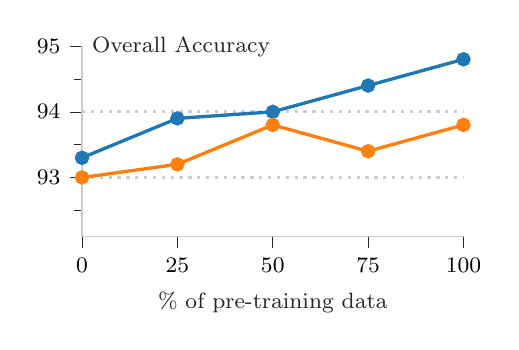
\begin{tikzpicture}

\definecolor{darkorange25512714}{RGB}{255,127,14}
\definecolor{darkslategray38}{RGB}{38,38,38}
\definecolor{lightgray204}{RGB}{204,204,204}
\definecolor{steelblue31119180}{RGB}{31,119,180}

\begin{axis}[
width=0.53\linewidth,height=4cm,
axis x line=bottom,
axis y line=left,
x axis line style={-},
ytick distance=0.5,
minor y tick num=1,
ytick={92, 93, 94, 95},
y axis line style={-},
axis line style={white!80!black},
legend cell align={left},
legend style={
  fill opacity=0.8,
  draw opacity=1,
  text opacity=1,
  at={(0.97,0.03)},
  anchor=south east,
  draw=lightgray204,
  legend image post style={line width =1.0pt}
},
tick align=outside,
xlabel=\textcolor{darkslategray38}{\footnotesize \% of pre-training data},
xmin=0, xmax=100,
xtick={0, 25, 50, 75, 100},
xtick style={color=darkslategray38},
y grid style={lightgray204},
x grid style={lightgray204},
every axis y label/.style={at={(0.001,1.1)},anchor=north west},
ylabel=\textcolor{darkslategray38}{\footnotesize Overall Accuracy},
ymin=92.1, ymax=95.0,
ytick style={color=darkslategray38},
tick label style={font=\footnotesize},
]

\addplot [very thick, dotted, lightgray204]
table {%
0 93
100 93
};

\addplot [very thick, dotted, lightgray204]
table {%
0 94
100 94
};

\addplot [very thick, steelblue31119180, mark=*, mark size=2, mark options={solid}]
table {%
0 93.3
25 93.9
50 94.0
75 94.4
100 94.8
};
\addplot [very thick, darkorange25512714, mark=*, mark size=2, mark options={solid}]
table {%
0 93.0
25 93.2
50 93.8
75 93.4
100 93.8
};

\end{axis}

\end{tikzpicture}}%
\hfill
\subcaptionbox{ScanObjectNN\,\cite{uy2019scanobjectnn}}{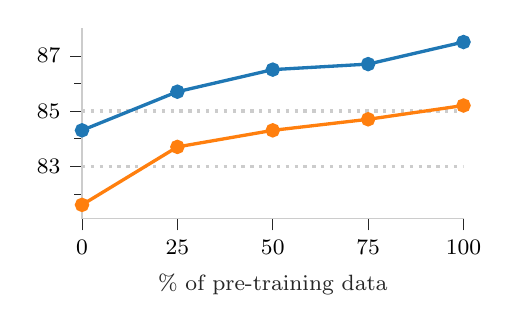
\begin{tikzpicture}

\definecolor{darkorange25512714}{RGB}{255,127,14}
\definecolor{darkslategray38}{RGB}{38,38,38}
\definecolor{lightgray204}{RGB}{204,204,204}
\definecolor{steelblue31119180}{RGB}{31,119,180}

\begin{axis}[
width=0.53\linewidth,height=4cm,
axis x line=bottom,
axis y line=left,
x axis line style={-},
ytick distance=0.5,
minor y tick num=1,
ytick={81, 83, 85, 87},
y axis line style={-},
axis line style={white!80!black},
legend cell align={left},
legend style={
  fill opacity=0.8,
  draw opacity=1,
  text opacity=1,
  at={(0.97,0.03)},
  anchor=south east,
  draw=lightgray204,
  legend image post style={line width =1.0pt}
},
tick align=outside,
xlabel=\textcolor{darkslategray38}{\footnotesize \% of pre-training data},
xmin=0, xmax=100,
xtick={0, 25, 50, 75, 100},
xtick style={color=darkslategray38},
y grid style={lightgray204},
x grid style={lightgray204},
every axis y label/.style={at={(0.001,1.0)},anchor=north west},
ymin=81.1, ymax=88.0,
ytick style={color=darkslategray38},
tick label style={font=\footnotesize},
]

\addplot [very thick, dotted, lightgray204]
table {%
0 83
100 83
};

\addplot [very thick, dotted, lightgray204]
table {%
0 85
100 85
};

\addplot [very thick, steelblue31119180, mark=*, mark size=2, mark options={solid}]
table {%
0 84.3
25 85.7
50 86.5
75 86.7
100 87.5
};
\addplot [very thick, darkorange25512714, mark=*, mark size=2, mark options={solid}]
table {%
0 81.6
25 83.7
50 84.3
75 84.7
100 85.2
};

\end{axis}

\end{tikzpicture}}%

\caption{
\textbf{Pre-training Data Efficiency.}
Irrespective of the quantity of pre-training data used from ShapeNet, \name{} consistently achieves better results than Point-MAE\,\cite{pang2022pointmae} on ModelNet40 (with voting) and the most difficult test split of ScanObjNN.
}
\label{fig:pretraining_data_efficiency}
\vspace{-20pt}
\end{figure}
We evaluate the efficiency of self-supervised pre-training with \name{}.
To this end, we partition the ShapeNet training dataset into subsets containing $25\%$, $50\%$, $75\%$ and $100\%$ of the data.
We then fine-tuned our model for shape classification on ModelNet40 and ScanObjectNN, respectively.
As shown in\,\reffig{pretraining_data_efficiency}, \name{} achieves consistent improvements on both datasets.
Notably, pre-training \name{} with only $25\%$ of the training data yields superior results compared to Point-MAE pre-trained with $100\%$ of the training data.

\paragraph{Class Confusions on ModelNet40.}
Given the very high overall accuracies on the ModelNet40 dataset, we further analyze the remaining errors.
\reffig{modelnet_confusion} shows the confusion matrix on the ModelNet40 test split, clearly showing that most remaining mistakes are made for a few classes with very similar appearances, which might also be difficult for humans to distinguish.


\section{Architecture Details.}


In \reftab{hyperparameters}, we provide detailed hyperparameters for pre-training \datavec{} and \name{} on ShapeNet.
We, furthermore, report the hyperparameters for fine-tuning \name{} for the shape classification (\reftab{hyperparameters_classification}) and part segmentation task (\reftab{hyperparameters_part_segmentation}).
In Listing \ref{lst:point2vec}, we provide the PyTorch-inspired pseudocode for \name{} pre-training.

\section{Qualitative Results for Part Segmentation.}
\begin{figure*}[t!]
\includegraphics[width=1.0\linewidth,trim={0cm 0.85cm 0cm 0.85cm},clip]{figures/shapenetpart_qualitative/part_qual.pdf}
\caption{
\textbf{Qualitative Results on ShapeNetPart.}
\name{} produces well localized boundaries between parts with minimal semantic errors.
In most cases, the differences between the results of \name{} and the ground truth are imperceptible to the human eye.
However, the last example shows a failure case where the jet engine is not properly segmented.
}
\label{fig:shapenetpart_qualitative}
\end{figure*}
In \reffig{shapenetpart_qualitative}, we show qualitative results for part segmentation on the ShapeNetPart dataset.
\emakefirstuc{\name{}} achieves remarkable results, as the boundaries between parts are accurately localized with minimal semantic errors.
In the majority of instances, there is no perceivable difference between the results produced by \name{} and the ground truth.




\begin{table}
    \centering
    \caption{
        \textbf{Hyperparameters for \datavec{} and \name{}.}
        \emakefirstuc{\datavec{}} denotes our adaptation of data2vec to the point cloud modality.
        We report the best performing hyperparameters for both \datavec{} and \name{}.
        LN: layer normalization. AVG: average pooling over layers.
    }
    \label{tab:hyperparameters}
    \begin{tabular}{lll}
        \toprule
        & \textbf{\datavec}                   & \textbf{point2vec}                        \\
        \midrule
        Steps                   & $800$ epochs                               & $800$ epochs                                \\
        Optimizer                                          & AdamW                                     & AdamW                                     \\
        Learning rate        & $2 \times 10^{-3}$                                & $1 \times 10^{-3}$                                \\
        Weight decay        & $0.05$                                      & $0.05$                                      \\
        LR Schedule  & cosine                                    & cosine                                    \\
        LR Warm-Up       & $80$ epochs                       & $80$ epochs                       \\
        Batch size            & $2048$                                      & $512$                              \\
        Encoder layers         & $12$                                        & $12$                                        \\
        Encoder dimension       & $384$                                       & $384$                                       \\
        Decoder layers           & --                                         & $4$                                         \\
        Masking strategy            & random                                    & random                                    \\
        Masking ratio                       & $65\%$ & $65\%$ \\
        \arrayrulecolor{black!10}\midrule\arrayrulecolor{black}
        $\tau_0$ (EMA start)  & $0.9998$                            & $0.9998$                              \\
        $\tau_e$ (EMA end)     & $0.99999$     & $0.99999$     \\
        $\tau_n$ (EMA warm-up)  & $200$ epochs                     & $200$ epochs                       \\
        $K$ (layers to average) & $6$                                         & $6$                                         \\
        Target normalization &     \small LN$\rightarrow$AVG$\rightarrow$LN         & \small LN$\rightarrow$AVG$\rightarrow$LN         \\
        \bottomrule
    \end{tabular}
\end{table}
\begin{table}
	\centering
	\caption{
		\textbf{Hyperparameters for Classification.}
            We use the same hyperparameters when fine-tuning \name{} and \datavec{} on ModelNet40\,\cite{wu2015modelnet40} and ScanObjectNN\,\cite{uy2019scanobjectnn}.
            When training from scratch, we increase the learning rate to $1 \times 10^{-3}$ and do not freeze the Transformer encoder.
	}
	\label{tab:hyperparameters_classification}
	\begin{tabular}{lll}
		\toprule
		Epochs                   & $150$ \\
		Batch size              & $32$                  \\
		Optimizer               & AdamW               \\
		Learning rate           & $3 \times 10^{-4}$  \\
		Weight decay            & $0.05$                \\
		Learning rate schedule  & cosine              \\
		Learning rate warm-up   & $10$ epochs           \\
  \arrayrulecolor{black!10}\midrule\arrayrulecolor{black}
            points & $1024$ \footnotesize($2048$ for ScanObjNN) \\
            $n$ (center points) & $64$ \footnotesize($128$ for ScanObjNN) \\
            $k$ ($k$-NN grouping) & $32$ \\
		mini-PointNet 1st MLP dim          & $128$, $256$                  \\
		mini-PointNet 2nd MLP dim          & $512$, $384$                  \\
  \arrayrulecolor{black!10}\midrule\arrayrulecolor{black}
		Encoder layers          & $12$                  \\
		Encoder dimension       & $384$                 \\
		Encoder heads           & $6$                 \\
		Encoder drop path           & $0\%,\ldots,20\%$                 \\
		Encoder frozen & $100$ epochs \\
  \arrayrulecolor{black!10}\midrule\arrayrulecolor{black}
            Feature aggregation & mean- \& max-pooling \\
            Classification head dim & $256$, $256$, \#classes \\
            Classification head dropout & $50\%$ \\
            Label smoothing & $0.2$ \\
		\bottomrule
	\end{tabular}
\end{table}

\begin{table}
	\centering
	\caption{
		\textbf{Hyperparameters for Part Segmentation.}
            We use the same hyperparameters when fine-tuning \name{} and \datavec{} on ShapeNetPart\,\cite{yi16siggraph}.
	}
	\label{tab:hyperparameters_part_segmentation}
	\begin{tabular}{lll}
		\toprule
		Epochs                   & $300$ \\
		Batch size              & $16$                  \\
		Optimizer               & AdamW               \\
		Learning rate           & $2 \times 10^{-4}$  \\
		Weight decay            & $0.05$                \\
		Learning rate schedule  & cosine              \\
		Learning rate warm-up   & $10$ epochs           \\
  \arrayrulecolor{black!10}\midrule\arrayrulecolor{black}
            points & $2048$ \\
            $n$ (center points) & $128$ \\
            $k$ ($k$-NN grouping) & $32$ \\
		mini-PointNet 1st MLP dim          & $128$, $256$                  \\
		mini-PointNet 2nd MLP dim          & $512$, $384$                  \\
  \arrayrulecolor{black!10}\midrule\arrayrulecolor{black}
		Encoder layers          & $12$                  \\
		Encoder dimension       & $384$                 \\
		Encoder heads           & $6$                 \\
		Encoder drop path           & $0\%,\ldots,20\%$                 \\
  \arrayrulecolor{black!10}\midrule\arrayrulecolor{black}
            Feature propagation & described in main paper \\
            Segmentation head dim & $512$, $256$, \#classes \\
            Segmentation head dropout & $50\%$ \\
		\bottomrule
	\end{tabular}
\end{table}

\begin{lstlisting}[language=Python, float=*t, caption=\textbf{PyTorch-inspired pseudocode for \name{} pre-training.}, label={lst:point2vec}, escapechar=!]
# N: batch size (512)
# S: number of groups/embeddings (64)
# E: embedding feature dimension (384)

for point_cloud in data_loader:
    # point cloud embedding
    center_points = self.FPS(point_cloud)  # (N, S, 3)
    # (N, S, 32, 3)
    point_patches = self.KNN(point_cloud, center_points)  
    # (N, S, E) (Fig. 2, !\colorsquare{m_pointnet}!)
    patch_embeddings = self.mini_pointnet(point_patches)  
    # (N, S, E)
    pos_embeddings = self.pos_encoder(center_points)  
  
    # masking
    # (N, S, E)
    mask_embeddings = self.mask_embedding.expand(N, S, E)  
    mask = generate_mask(center_points)  # (N, S) boolean
  
    # targets
    with torch.no_grad():
        # (12, N, S, E) (Fig. 2, !\colorsquare{m_green}!)
        teacher_states = self.teacher(patch_embeddings, 
                                      pos_embeddings)  
        target_layers = [F.layer_norm(x, (E,)) for x in 
                         teacher_states[6:]]  # [(N, S, E)]
        targets = torch.stack(target_layers).mean(0) # (N, S, E)
        targets = F.layer_norm(targets, (E,))  # (N, S, E)
        
    # predictions
    last_student_state = self.student(  # (N, S, E) (Fig. 2, !\colorsquare{m_blue}!)
        patch_embeddings[~mask].reshape(N, -1, E),
        pos_embeddings[~mask].reshape(N, -1, E)
    )[-1]
    predictions = self.decoder(  # (N, S, E) (Fig. 2, !\colorsquare{m_red}!)
        mask_embeddings.index_put([~mask], 
        last_student_state.reshape(-1, E)),
        pos_embeddings
    )[-1]
  
    # optimization
    loss = F.smooth_l1_loss(predictions[mask], targets[mask])
    loss.backward()
    optimizer.step()
  
    # update teacher weights
    ema_update(student, teacher)
\end{lstlisting}


\end{document}
